\cleardoublepage
\section{Example tutorial case results}
\label{sec:exp}

In the present section the results of the chosen example tutorial case are presented. The simulation of the flow, and the air pollution spreading are performed in the segregated manner. 

Firstly, we focus onto the flow results, i.e.\ the solution of the~(\ref{eq:RANS1},~\ref{eq:RANS2}). The simulation run in parallel utilizing 12 cores of the Taiwania-3 server~\cite{tw3} for approximately 4 hours.  The resulting stream-wise velocity component contours ($u_x$) on the $y$-normal slice, and the pressure contours ($p$) on the ground computational domain boundary ($\partial\Omega_{\mathrm{g}}$) are presented in Figure~\ref{fig:ux_p}. 

\begin{figure}[htpb]
    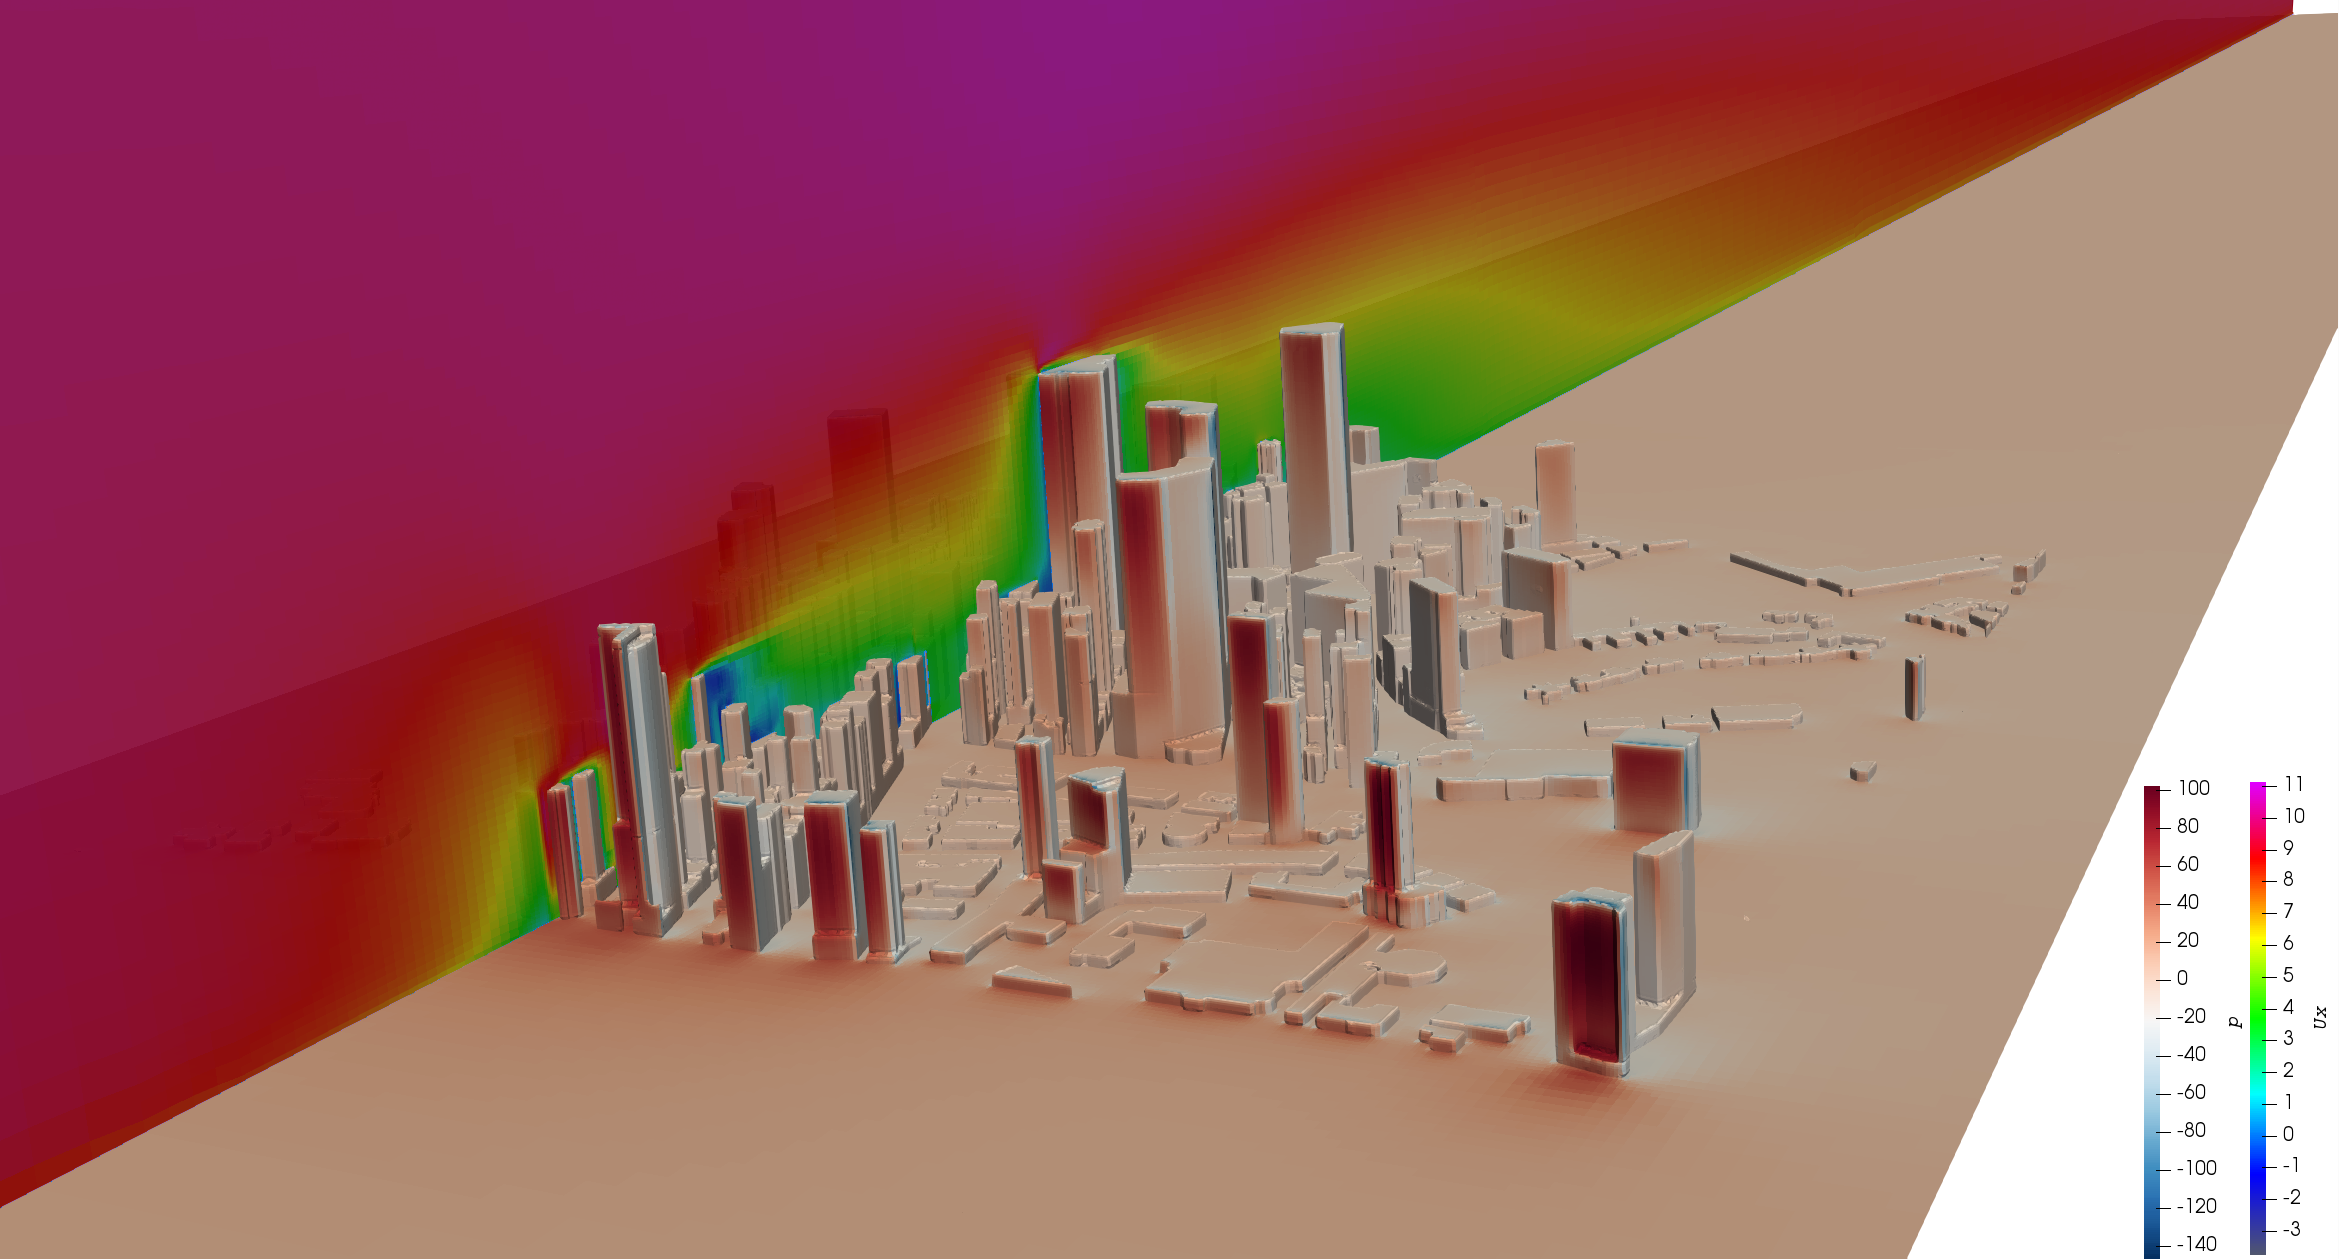
\includegraphics[width=0.95\textwidth]{01_images/res/pUxFront2.png}
    \caption{Stream-vise velocity component ($u_x$), and pressure ($p$) contours on $y$-normal slice, and the ground boundary, respectively.}
    \label{fig:ux_p}
\end{figure}

With the 